\chapter{Implementation}

As we repeatedly mentioned in the first chapter, the design we chose should allow multiple implementations for each module. The implementations provided in this thesis are designed for use-cases ranging from beginner user that requires only core functionality to advanced users who can utilize full module distribution. The resulting implementation therefore offers a monolithic application as well as separate modules.
\par
In this chapter we will discuss the implementation details of every module. At the beginning we will explain our programming language choices. We will add a short description for every library that we used and a reason why we preferred it to others.

%%-----------------------------------------------------------------------------------------
%% SECTION
%%-----------------------------------------------------------------------------------------
\section{Programming Language}

First decision we had to take was to select a suitable programming language. We had to follow the main guidelines that we have set earlier. That is, we had to find a way to support multiple platforms, while in the same time we needed flexible enough language to handle our modular design and fast enough to help us with scalability.
\par
Even though our modules are separable and therefore each of them could be written in a different language, we wanted to reduce the amount of used languages to minimum, ideally just one or two for the sake of simplicity. Furthermore, we focused on languages that would allow us to write one implementation for all platforms with the minimum of tweaks. Last but not least, we wanted a language that we had at least some experience with.
\par
We have narrowed the choice to three possible main programming languages for our implementation: C++, C\# and Java. All of them are major languages, have cross-platform capabilities and are well-established with enough libraries for all our features. We excluded popular languages Python and JavaScript due to their nature as scripting languages and therefore not providing enough performance for a bigger scale project.

%%-----------------------------------------------------------------------------------------
\subsection{GUI struggles}

The weak spot of all three languages is graphical user interface~(GUI) necessary for our Manager module. We would like the module to be modern and visually attractive and common GUI frameworks are usually either platform-specific, difficult to work with or have too many limitations. The exception might be
Qt~\citep{qt}, which is a very capable GUI toolkit written in C/C++, plus there is a Java wrapper for this library available.
\par
In the past few years, web applications have become very popular. Increasing performance of personal computers and development in web technologies as well as rise of single-page application frameworks allowed the creation of applications running almost entirely in a web browser. Nowadays, many people use only web browser on their computer where they have access to all sorts of web applications for any purpose. This has also changed their perception of how user interface should look like. Following this trend there are some desktop applications written entirely using web technologies, enclosed in a web browser wrapper.
\par
We decided to adopt above-mentioned approach for our Manager module. There is an open-source project written in C++ called Chromium Embedded Framework~(CEF). CEF focuses on facilitating embedded browser use cases in third-party applications~\citep{cef}. It means that we can create GUI using HTML5 and JavaScript relying on flexibility, cross-platform support and relative simplicity that they provide compared to other options. CEF offers a way to call C++ code from JavaScript so we can further customize its behavior as a proper desktop application.
\par
It is important to note that this decision was influenced by the desire to provide both modular as well as monolithic-looking application. Web GUI can be written once and then be utilized as a stand-alone module running on any web browser or wrapped as desktop application using CEF. Moreover, we can extend it using C++ to bundle it up with the remaining modules and create all-in-one application. Finally, it integrates well with our Database module as Firebase provides its SDK in JavaScript.

%%-----------------------------------------------------------------------------------------
\subsection{Final decision}

Having chosen a programming language and additionally a framework for Manager module, it remains to choose it for Player and Fileserver modules. Out of the three preselected languages we made C++ our final decision.
Both other languages would be equally capable for the task, but C++ provides more performance and more control of memory management. Furthermore, it does not rely on a virtual machine and is already utilized within our Manager module. Lastly, these two modules contain a lot of low-level programming, what makes C++ a preferable candidate and a lot of related libraries are written directly in C/C++.

%%-----------------------------------------------------------------------------------------
%% SECTION
%%-----------------------------------------------------------------------------------------
\section{Fileserver Module}

This module consists of two main parts - file storage and RESTful interface. We used SQL database to store music file metadata and its location in file system and playlists. The REST API follows predefined interface. It adds additional resources for file management as its selected way to manage content.

\subsection{Libraries used}
We used two third-party libraries for the implementation of this module.
\par
First one is SQLite that we used for data storage. SQLite is a C-language library that implements a small, fast, self-contained, high-reliability, full-featured, SQL database engine. SQLite is the most used database engine in the world. SQLite is built into all mobile phones and most computers and comes bundled inside countless other applications that people use every day. The SQLite file format is stable, cross-platform, and backwards compatible and the developers pledge to keep it that way through at least the year 2050. SQLite database files are commonly used as containers to transfer rich content between systems and as a long-term archival format for data. There are over 1 trillion SQLite databases in active use~\citep{sqlite}. It allows us to to create a small SQL database file locally on the device where it runs.
\par
The other library we used is called C++ REST SDK~(cpprestsdk). The C++ REST SDK is a Microsoft project for cloud-based client-server communication in native code using a modern asynchronous C++ API design. This project aims to help C++ developers connect to and interact with services. Microsoft have developed this library, because historically C++ developers have been lacking a basic set of tools that enable them to access and author REST services in a productive, scalable and asynchronous manner. C++ Rest SDK aims to alleviate some of the pain felt by developers by providing a cross-platform library that is modeled on simplicity, extensibility and composition~\citep{cpprestsdk}. Even though C++ is not a preferred language for creating REST services, this library offers a simple way for both creating and accessing these services. It handles the network communication for us and allows us to focus on the business logic that processes and delivers data.
\todo{maybe add that their are open source and cross platform? mention troubles with cpprestsdk?}

%%-----------------------------------------------------------------------------------------
\subsection{Data Storage}
Usually, all song files contain metadata besides the actual music data. They contain information such as song title, author, album, or genre and are stored in a data structure called tag. Reading it from the file repeatedly is hugely ineffective so we read them only once when the file is added to the library. After that, we need to store it somewhere along with the path to the file, as they may be scattered across the file system.
\par
There are multiple possibilities of how to store it. The API requires the ability to search in the library so the common approach would be to store the data in a relational database. This implementation is intended to support a single or up to just a couple of users - its purpose is to allow users to create their own music library. Therefore, utilizing a dedicated database server is unreasonable. Instead, we used SQLite library as it provides a full-featured SQL database engine in a single library. It can easily store thousands of records which is sufficient.

%%-----------------------------------------------------------------------------------------
\subsubsection{Code Remarks}
In the code, we created a single class that takes care of working with the database. We named it \texttt{SqliteAPI}, as it provides an API for working with our SQLite library. This class handles SQL query creation and communication with database. Since all its methods are called from REST API calls, they all return an error code so in case an error occurred it can be reported to caller. The actual return value is then passed in a form of out parameter. Methods that retrieve data accept a list of parameters that allow filtering and modifying the results of their query.
\par
Additionally, this class contains functionality for adding new music files to library. It utilizes tinyfiledialogs library to display cross-platform file dialogs to allow users to choose new files. To extract metadata from these files we used ffmpeg library. We will talk further about this library in the Player Module section \todo{forward referencia, skusit vymysliet inak} where we utilize it for decoding. Here, we used its capability to read music files and retrieve metadata which are then stored in the database. This functionality is wrapped in \texttt{AudioInspector} class.

%%-----------------------------------------------------------------------------------------
\subsubsection{Database Schema}
\begin{figure}[ht]\centering
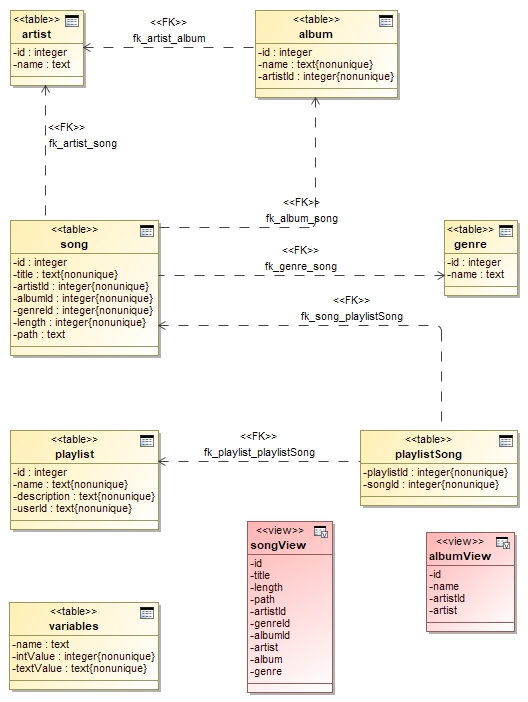
\includegraphics[width=1.0\textwidth]{img/DbDiagram2.png}
\caption{Database schema}
\label{fig03:dbSchema}
\end{figure}

%%-----------------------------------------------------------------------------------------
\subsection{Rest API}
Creating a REST API in C++ was not an easy task. There are many more suitable programming languages for that. However, C++ REST SDK library provides a lot of tools to make it easier than integrating with an API written in a different language. It provides a HTTP listener that listens for incoming requests and a set of asynchronous methods to handle these requests in a modern and effective way. For this, it provides its own implementation of asynchronous tasks.

%%-----------------------------------------------------------------------------------------
\subsubsection{Code Remarks}
To create an abstraction between the HTTP listener and data storage we utilized the bridge design pattern. It allowed us to create HTTP listener independent from data storage. Coupling it with another data storage would just require implementing the abstract class \texttt{AbstractFileServerHandler} in a new bridge.
\par
The \texttt{FileServerAPI} class is the implementation of the mentioned listener. It listens for HTTP requests on chosen address and port. It supports \texttt{GET}, \texttt{POST}, \texttt{PUT} and \texttt{DELETE} request methods required by Fileserver API design and adds \texttt{OPTIONS} method to provide cross-origin resource sharing~(CORS) headers. These are important to allow Manager module running on a browser that restricts cross-origin HTTP requests to access this API. Upon receiving a request a corresponding method handler parses and verifies the URI and parameters to determine the resource. Then it passes the parameters to a correct method of the associated bridge which executes the action and returns payload for the response. This response is then sent back to the client.
\par
\texttt{FileServerHandler} class is the bridge implementation for SQLite data storage. This bridge is the owner of \texttt{SqliteAPI} instance and translates REST API calls to \texttt{SqliteAPI} calls and translates data returned by \texttt{SqliteAPI} to JSON format supported by REST API.

\subsection{Security}
\todo{discuss a bit about security and what were the options and what did we choose to follow}

%%-----------------------------------------------------------------------------------------
%% SECTION
%%-----------------------------------------------------------------------------------------
\section{Player Module}

The main feature of Player module is playing music. Besides that, it is important to have music files ready for playback as they might not be stored on the same device. We implemented simple but reliable caching functionality to provide us with reliable amount of the files on demand. Lastly, we implemented a required WebSocket-based communication interface.

%%-----------------------------------------------------------------------------------------
\subsection{Libraries used}
We utilized three third-party libraries in this module. Two are used for audio playback and one for communication interface.
\par
FFmpeg is the leading multimedia framework, able to decode, encode, transcode, mux, demux, stream, filter and play pretty much anything that humans and machines have created. It supports the most obscure ancient formats up to the cutting edge. No matter if they were designed by some standards committee, the community or a corporation. It is also highly portable: FFmpeg compiles, runs, and passes testing infrastructure FATE across Linux, Mac OS X, Microsoft Windows, the BSDs, Solaris, etc. under a wide variety of build environments, machine architectures, and configurations~\citep{ffmpeg}. Basically, this library allows us to support any music file format we  would like to. We utilised it in Fileserver module for metadata extraction, but it is utilised more heavily here for audio decoding.
\par
To output decoded audio to speakers, we used PortAudio library. PortAudio is a free, cross-platform, open-source, audio I/O library. It lets you write simple audio programs in 'C' or C++ that will compile and run on many platforms including Windows, Macintosh OS X, and Unix (OSS/ALSA). It is intended to promote the exchange of audio software between developers on different platforms. Many applications use PortAudio for Audio I/O~\citep{portaudio}. This library offers cross-platform access to audio I/O as all platforms have their own way of working with it.
\par
Even though C++ REST SDK that we used in Fileserver module promises WebSocket functionality, it only supported WebSocket client at the time. We need to build a WebSocket server so we had to choose different library. For this task we chose Boost.Beast library. Beast is a C++ header-only library serving as a foundation for writing interoperable networking libraries by providing low-level HTTP/1, WebSocket, and networking protocol vocabulary types and algorithms using the consistent asynchronous model of Boost.Asio~\citep{beast}. While this library provides low-level tools, we needed to build just a small server so it allowed us to customize it to create simple and small implementation with the benefits of asynchronous programming from Boost.Asio library.
\todo{write about boost, ffmpeg and portaudio}

%%-----------------------------------------------------------------------------------------
\subsection{File Caching}

The requirements for file caching from analysis are to support two queues and to have a full song ready for playback while another finishes. The second one is important to provide smooth playback without pauses for buffering. We had two options where to store the cached songs - in memory or on hard drive. We decided to store it in memory.
\par
The hard drive option would allow us to cache more songs. That would allow the application to work better on places with slower or less stable internet connection. On the other hand, it is much slower first to store the data and then to decode it, just to delete it afterwards. Additionally, SSD drives and flash memories that are becoming more popular recently do not handle such frequent writes very well and frequent usage of our application would wear these drives down too early.
\par
Storing cached music files in memory reduces the amount of data transfers and files are instantly ready for decoding. However, we can not store too many files as miniature PCs, that might be utilised by this module, do not have too much memory space to spare. Therefore we cache only two files at once in each queue plus one that is being played, 5 in total. When a song is dequeued for playback a new one gets cached, so by the time it finishes there are two songs prepared again. With estimated average size of a music file using compressed file format to be 10MB, we would require around 50MB for our cache. That should not create any problems. Even using lossless file formats where file sizes are around 70MB we would need only 350MB - a machine with 1GB RAM space should handle this module easily.
\par
This solution is volatile to frequent skipping of songs as big music files take time to get cached. However, this application is intended to provide continuous music playback without supervision and skipping songs should be used just as a tool to deal with malicious behavior such as ordering same song multiple times.

%%-----------------------------------------------------------------------------------------
\subsubsection{Code Remarks}

Cache is represented by \texttt{SongCache} class. This class implements all logic required for caching songs. It contains HTTP client from C++ REST SDK library that it uses to download music files to cache. Furthermore, it implements the algorithm for choosing the next song defined in first chapter. It provides two inputs for song queues and outputs next song to be played. Cache is bound to a certain Fileserver module defined upon its creation. It can be reset to clear its contents, but to bind to a new Fileserver, one needs to create a new instance.
\par
Internally, \texttt{SongCache} utilizes \texttt{SongCacheItem} class for storing each queued item. This class holds an asynchronous buffer that is used to download the data asynchronously and upon completion it provides a \texttt{std::basic\_istream} for reading cached file contents. Before accessing it, it is necessary to check for errors.

%%-----------------------------------------------------------------------------------------
\subsection{Communication Protocol}

This module should support communication channel over WebSocket to communicate with Manager module. Player module has the role of server that listens and awaits connection from a Manager module. For that purpose we implemented a simple server that listens for incoming connections. Upon receiving a WebSocket handshake, a session is started and the server stops listening for more connection attempts until the session ends. Within a session, Manager and Player module exchange RPC messages encoded in JSON. The incoming message is checked for validity and then processed. Extracted parameters, if any, are passed to the correlating method, which is then invoked. If it needs to send one or more messages back, they are buffered and sent after the method finishes. To provide some defense against abuse there is a mechanism that ends the session after three consecutive invalid messages. 

%%-----------------------------------------------------------------------------------------
\subsubsection{Code Remarks}

The functionality of the server is layered into multiple classes. At the top is the \texttt{API} class. This class wraps the entire server and technically also the entire module functionality, as whole module is controlled directly through this communication protocol. It offers methods to start and stop the server.
\par
When the server is started, \texttt{API} class instance runs an instance of \texttt{Listener} class. This class provides functionality to listen for and accept incoming connections asynchronously.
\par
After a new connection is accepted, an instance of \texttt{Session} class takes over the created socket and handles the incoming ant outgoing communication. It represents a session of Player module during which the music playback occurs. This instance owns song cache and music player and takes care of cooperation between them. Reads and writes on WebSocket are performed asynchronously.

%%-----------------------------------------------------------------------------------------
\subsection{Audio Decoding and Playback}
\todo{explain how ffmpeg communicates with portaudio and all other things}
\todo{add some information about how are files encoded, formats, loss-less etc.}

%%-----------------------------------------------------------------------------------------
\subsection{Security}
\todo{discuss a bit about security and what were the options and what did we choose to follow}

%%-----------------------------------------------------------------------------------------
%% SECTION
%%-----------------------------------------------------------------------------------------
\section{Manager Module}
\todo{add short intro about how we designed it}

\subsection{Libraries used}
\todo{write about React, CEF, MaterialUI, intl, and maybe axios}

\subsection{Design Principles}
\todo{explain what principles we held during implementation, dumb and smart components, global state, action creators, reducers, routes}

%%-----------------------------------------------------------------------------------------
%% SECTION
%%-----------------------------------------------------------------------------------------
\section{Realtime Database Module}
\todo{add short intro about how we designed it}

\subsection{Structure}
\todo{describe firebase structure}